\documentclass[12pt,preprint]{aastex}
\usepackage{natbib,amsmath}
\special{papersize=8.5in,11in}
\begin{document}


\def\nhdlls{154}
\def\ntot{16X}
\def\npair{XX}
\def\nslls{99}
\def\hub{h_{72}^{-1}}
\def\umfp{{\hub \, \rm Mpc}}
\def\mew{W_\lambda}
\def\ew{$\mew$}
\def\mzq{z_q}
\def\mfmin{f_{\rm min}}
\def\fmin{$\mfmin$}
\def\zabs{$z_{\rm abs}$}
\def\mzabs{z_{\rm abs}}
\def\msna{{\rm S/N}^{\rm A}_{912}}
\def\sna{S/N$^{\rm A}_{912}$}
\def\mnull{\nu_{\rm 912}}
\def\nnull{$\nu_{\rm 912}$}
\def\intl{\int\limits}
\def\nstatqso{193}
\def\maxoff{0.4}
\def\clls{1.9 \pm 0.2}
\def\alls{5.2 \pm 1.5}
\def\blls{-0.9^{+0.4}_{-0.05}}
\def\cmma{\;\;\; ,}
\def\perd{\;\;\; .}
\def\ltk{\left [ \,}
\def\ltp{\left ( \,}
\def\ltb{\left \{ \,}
\def\rtk{\, \right  ] }
\def\rtp{\, \right  ) }
\def\rtb{\, \right \} }
\def\sci#1{{\; \times \; 10^{#1}}}
\def \rAA {\rm \AA}
\def \mzem {z_{\rm em}}
\def\smm{\sum\limits}
\def \cmm  {cm$^{-2}$}
\def \cmmm {cm$^{-3}$}
\def \kms  {km~s$^{-1}$}
\def \mkms  {{\rm km~s^{-1}}}
\def \lyaf {Ly$\alpha$ forest}
\def \Lya  {Ly$\alpha$}
\def \lya  {Ly$\alpha$}
\def \mlya  {Ly\alpha}
\def \Lyb  {Ly$\beta$}
\def \nhi  {$N_{\rm HI}$}
\def \mnhi  {N_{\rm HI}}
%\def \mtotnhi  {\mnhi^{\rm TOT}}
%\def \totnhi  {$\mtotnhi$}
\def \lnhi {$\log N_{HI}$}
\def \mlnhi {\log N_{HI}}
\def \etal {\textit{et al.}}
\def \ob {$\Omega_b$}
\def \obh {$\Omega_bh^{-2}$}
\def \om {$\Omega_m$}
\def \ol {$\Omega_{\Lambda}$}
\def \gz {$g(z)$}
\def \mgz {g(z)}
\def \lyaf {Lyman--$\alpha$ forest}
\def \fnhi {$f(\mnhi,X)$}
\def \mfnhi {f(\mnhi,X)}
%\def \llsteff {$\tilde\mtll$}
%\def \mllsteff {\tilde\mtll}
\def \mnmin {\mnhi^{\rm min}}
\def \nmin {$\mnhi^{\rm min}$}
\newcommand{\cm}[1]{\, {\rm cm^{#1}}}
\def\N#1{{N({\rm #1})}}
\def\psol#1#2#3#4{$\{ {\rm #1}^{#2}/{\rm #3}^{#4}\}$}
\def\pxh{$\{ {\rm X/H} \}$}
\def \snrlim {SNR$_{lim}$}
\def\mglls {\gamma_{\rm LLS}}
\def\mavgt {<\mtll>}

\title{igmspec
[v1.2]}

\author{
J. Xavier Prochaska\altaffilmark{1}, 
%John M. O'Meara\altaffilmark{2}, 
%Michele Fumagalli
%Rebecca A. Bernstein\altaffilmark{1} 
%Scott Burles\altaffilmark{3},
}
\altaffiltext{1}{Department of Astronomy and Astrophysics, UCO/Lick Observatory, University of California, 1156 High Street, Santa Cruz, CA 95064}
%\altaffiltext{2}{Department of Chemistry and Physics, Saint Michael's College.
%One Winooski Park, Colchester, VT 05439}
%\altaffiltext{3}{Visiting Astronomer, Las Campanas Observatory}

\begin{abstract}
igmspec 
\end{abstract}


%\keywords{absorption lines -- intergalactic medium -- Lyman limit systems -- SDSS}

\section{Introduction}
\label{sec:intro}

Shortly after the discovery of quasars by \cite{schmidt6X},
astronomers identified absorption-line features in their 
spectra indicating the presence of intergalactic gas
\citep{burbidge,bahcall}.  
The community quickly recognized both the value of these
data to cosmology and galaxy formation \cite{bahcall,spitzer}.
In the decades that followed, observationalists gathered
spectra of increasingly higher quality of several tens of
high-$z$ sources to analyze the IGM 
\citep{sargent,young,tytler,wolfe,lanzetta,bergeron}.
These were obtained primarily with private observatories and
the actual spectra were rarely made available
to the community.
An obvious exception was the data archives of the
{\it IUE} and {\it HST}  \citep{jannuzi,bechtold},
but even these were difficult to 
collate and combine.
One also recognizes the policy of ESO to archive and
make public their Very Large Telescope (VLT) datasets.

The past $\approx 10$\,years has witnessed the
rise of large, public spectral datasets especially
the 2dF and SDSS surveys \citep{york,2dF}.
This includes the spectra of several hundred thousand quasars
probing the IGM \citep{sdss_dr7Q,boss_dr12Q}.
These surveys have, in part, stimulated the public release
of smaller spectroscopic surveys with higher quality
(S/N, resolution) and/or complimentary sources
\citep[e.g.][]{pro07,hdlls}.
Accessing both the large survey datasets 
and these modest datasets of IGM spectroscopy
has remained a challenge, however, due to the lack of a
uniform standard in data format and distribution within the astronomical
community\footnote{This speaks to a general failure of the
Virtual Observatory.}
Ironically, this holds despite the fact that the reduced and calibrated
spectra probing the IGM comprise less than a few
tens Gb of disk space.

Therefore, as a service to the IGM researchers, ourselves, and the
broader community, we have initiated an effort to collate 
all of the published surveys of IGM spectroscopy. We distribute
these together with a simple software package
for accessing and manipulating the data.  
Termed {\it igmspec}, this database
is intended to grow with future surveys (e.g. DESI)
and to continue to ingest other historical 
datasets that come to light in
the public domain.  In addition, we provide 
software to generate private databases in tandem
with {\it igmspec}.  This may be of interest for surveys 
under construction, i.e.\ prior to publication.

This paper describes version v02 of the {\it igmspec}
database.  The manuscript is organized as follows:
Section~\ref{sec:catalog} describes the catalogs
included in {\it igmspec}.
Section~\ref{sec:datasets} details the spectral datasets
in {\bf v02} of {\it igmspec}.



\section{{\it igmspec} Catalog}
\label{sec:catalog}

At the heart of {\it igmspec} is a catalog of all sources,
each of which uniquely probes the IGM.
Each source is assigned a unique identifier IGM\_ID to be
preserved in all future versions of the database.\footnote{If a source
is discovered to be erroneous in the future, 
we will remove it without modifying
any other IGM\_ID values.}
To construct the catalog, we followed these steps:

\begin{enumerate}
\item Ingest all quasars from the BOSS DR12 survey.\footnote{See
http://www.sdss.org/dr12/algorithms/boss-dr12-quasar-catalog/}
\item Add all quasars from the SDSS DR7 survey not observed by BOSS.
These were defined as any sources with $\theta > 2''$ angular separation
from the BOSS dataset.
\item Add any additional, unique sources ($\theta > 2''$)
from the {\it igmspec} datasets.
\end{enumerate}
We then examined each pair of sources with $\theta \le 10''$ 
(\npair\ total) to establish if these are truly unique
The {\it igmspec} catalog includes a bare minimum of meta data
to limit its size and maximize search speed.
The ``keys'' are described in Table~\ref{tab:cat_keys}.

 
\begin{deluxetable}{lcl}
%\rotate
\tablewidth{0pc}
\tablecaption{CATALOG META DATA KEYS\label{tab:cat_keys}}
\tabletypesize{\scriptsize}
\tablehead{\colhead{Key} & \colhead{Type} 
& \colhead{Description}
}
\startdata
RA           & float64 & Right Ascension in J2000 (degrees) \\
DEC          & float64 & Declination in J2000 (degrees) \\
IGM\_ID      & int     & Unique {\it igmspec} identifier \\
flavor       & str     & Type of source (quasar, GRB, galaxy) \\
zem          & float64 & Redshift of the source \\
sig\_zem     & float64 & Uncertainty in the source redshift \\
flag\_zem    & int     & Flag describing the redshift measurement \\
flag\_survey & int     & Bitwise flag indicating the surveys covering the source \\
\enddata
%\tablecomments{All column densities are log$_{10}$. When the reported $\sigma=+9.99$, }
\end{deluxetable}

In addition to the {\it igmspec} catalog, we include the quasar
catalog compiled, maintained, and kindly shared by A. Myers.
See the documentation for a description of the priority given to 
redshift measurements collated in that catalog.


\section{{\it igmspec} Datasets}
\label{sec:datasets}

This manuscript describes the second version of the {\it igmspec}
database and represents our first comprehensive effort to collate
spectra probing the IGM at UV and optical wavebands at all
redshifts.  Future efforts will extend to other wavebands and/or
additional types of sources 
\citep[e.g. star-forming galaxies][]{rubin+14,rubin+16}.

Table~\ref{tab:datasets} lists the surveys included in
{\it igmspec\_v02} and briefly summarizes key aspects
of each survey.  The {\it igmspec} documentation and 
the original references provide greater detail on the meta data
and spectra included within each survey but the following
sub-sections also provide a brief description of each.

\begin{deluxetable}{lcl}
%\rotate
\tablewidth{0pc}
\tablecaption{SPECTRAL DATASETS\label{tab:datasets}}
\tabletypesize{\scriptsize}
\tablehead{\colhead{Dataset} & \colhead{Type} 
& \colhead{Description}
}
\startdata
Make & Auto & Matically \\
\enddata
%\tablecomments{All column densities are log$_{10}$. When the reported $\sigma=+9.99$, }
\end{deluxetable}

\subsection{BOSS DR12}

The Baryonic Oscillations Spectroscopic Survey (BOSS)
observed several hundred thousand quasars as part of its
primary survey.  With its final, complete data release
(DR12), the BOSS team provided several catalogs of quasars
observed in the main survey.  We have drawn from the three
catalogs at their main website.\footnote{http://www.sdss.org/dr12/algorithms/boss-dr12-quasar-catalog/}


The BOSS spectra bundled in {\it igmspec\_v02} were pulled
from the main data server and correspond to the
v5\_7\_0 data reduction.
[How about masked pixels?]

In addition to the calibrated spectra, we include a
continuum estimate for each quasar.  For wavelengths
long-ward of the quasar's \lya\ emission we adopt
the model generated by G. Zhu 
\citep[see][for details on the algorithm]{zhu15}.
For XXX quasars analyzed by \cite{lee1X} for an assessment
of the flux probability distribution function of the 
\lya\ forest, we adopt their mean-flux-regulated continua
\citep{lee1Xb}.

%
\subsection{SDSS DR7}
\label{sec:dr7}

The Sloan Digital Sky Survey observed over 100,000 quasars
as part of the SDSS-I survey.  These were primarily targeted
based on their optical photometry.  In 2011, one of us
performed an SQL query of the SDSS database to retrieve\footnote{GIVE SQL}
all spectroscopic sources classified as a QSO or HIZ\_QSO. 
This generated a list of 102,418 sources.  

We caution that several of these sources are mis-classified
as quasars, especially the anamolously bright ones at $z>4$.
To restrict to bona-fide quasars, we cross-matched this
sample against the \cite{meyers1X} quasar catalog.
[Schneider too]

\subsection{KODIAQ DR1}
\label{sec:kodiaq}

The Keck Observatory Database of Ionized Absorption toward Quasars (KODIAQ) survey is a public spectra data release of quasars observed with the HIRES spectrometer 
\citep{vogt94} on the Keck~I telescope. 
The first Data Release (DR1) became available in 2015, 
as described in \cite{kodiaq_dr1}. 
We have ingested the complete DR1 dataset.

\subsection{HD-LLS DR1}
\label{sec:hdlls}

The high dispersion Lyman Limit System (HD-LLS) sample is a set of echelle and echellette spectra described by \cite{hdlls}.  These were primarily acquired
to perform an analysis of $z \sim 3$ LLS. 
The quasars are a heterogeneous set of sources useful for such 
analysis (i.e.\ bright).

\subsection{GGG}
\label{sec:ggg}

The Giant Gemini GMOS (GGG) survey is a spectroscopic survey of 
$z>4.4$ quasars drawn from the Sloan Digital Sky Survey and re-observed with the GMOS spectrometer on the Gemini North and South telescopes. 
The data release is described in \cite{worseck+14}.


%%%%%%%%%%%%%%
\section{{\it igmspec} Architecture}
\label{sec:arch}

The {\it igmspec} database is provided as a single HDF5 file
containing both the catalogs and the survey spectral data.  
Each survey comprises an HDF5 Group
with a {\it meta} Dataset and a {\it spec} Dataset.
The former is an {\tt astropy} Table, with one row per
spectrum, converted into an HDF5 object.
The latter is an {\tt numpy.ndarray} 
with dtype names `wave', `flux', and `sig' for the
wavelength, flux, and $1\sigma$ error arrays.
Some surveys also include `co' for an estimate of the source
continuum.  

The HDF5 format enables rapid access to the data without
reading the entire database into memory.  
Figure~\ref{fig:arch} illustrates the 
architecture of the HDF5 file.


\section{{\it igmspec} Software}
\label{sec:software}

A modest set of Python modules and scripts are provided
with the {\it igmspec} database.  This includes a simple
script {\tt get\_igmspec} to download the latest
(or any previous) version of the database.
Additional software enables the user to plot an
input source, examine meta data, and do simple queries.

The IgmSpec class provides a lightweight object for
interfacing with the catalog and spectroscopic datasets
from within Python.  See the iPython Notebook\footnote{
https://github.com/pyigm/igmspec/blob/master/docs/examples/Simple\_Usage.ipynb}
for simple usage cases.

All of the software is provided in a git repository\footnote{
https://github.com/pyigm/igmspec}
and is being actively developed by the community.

\section{Concluding Remarks}
\label{sec:end}

With {\it igmspec}, it is our goal to provide (nearly)
all of the published spectral datasets that effectively
probe the IGM.  Hopefully, this effort will
enable new, unforeseen research on the IGM as well
as the greater diffusion of otherwise difficult-to-access spectral
datasets.  

In {\bf v03} of
{\it igmspec}, we plan to include at least the following:
(1) additional near-IR spectroscopy;
(2) radio absorption spectra \citep[e.g. 21\,cm][]{kanekar1X};
(3) galaxy spectra probing the IGM \citep[e.g.][]{rubin+16}.
Community members interested in guiding the future development
of {\it igmspec} are encouraged to contribute via github
(https://github.com/pyigm/igmspec).

To enable IGM cross-correlation analyses with galaxies
and the large-scale structures they trace,
we intend the future release of {\it exgalspec}.
This database will have -- at
the minimum -- a catalog of (nearly) all spectroscopically
confirmed galaxies and, where feasiable, their associated
spectra.  See https://github.com/pyigm/exgalspec
to contribute to that effort.


\acknowledgments

J. X. P. was supported by NSF grant AST-1412981.
We thank JMO, GW, JR, NM
%J.X.P and G.W. are partially supported
%by an NSF CAREER grant (AST--0548180), and 
%by NSF grant AST-0908910.


%\bibliographystyle{/u/xavier/paper/Bibli/apj}
%\bibliography{/u/xavier/paper/Bibli/allrefs}

%\input{Tables/tab_HIRES.tex}
%\input{Tables/tab_MIKE.tex}


\begin{figure}
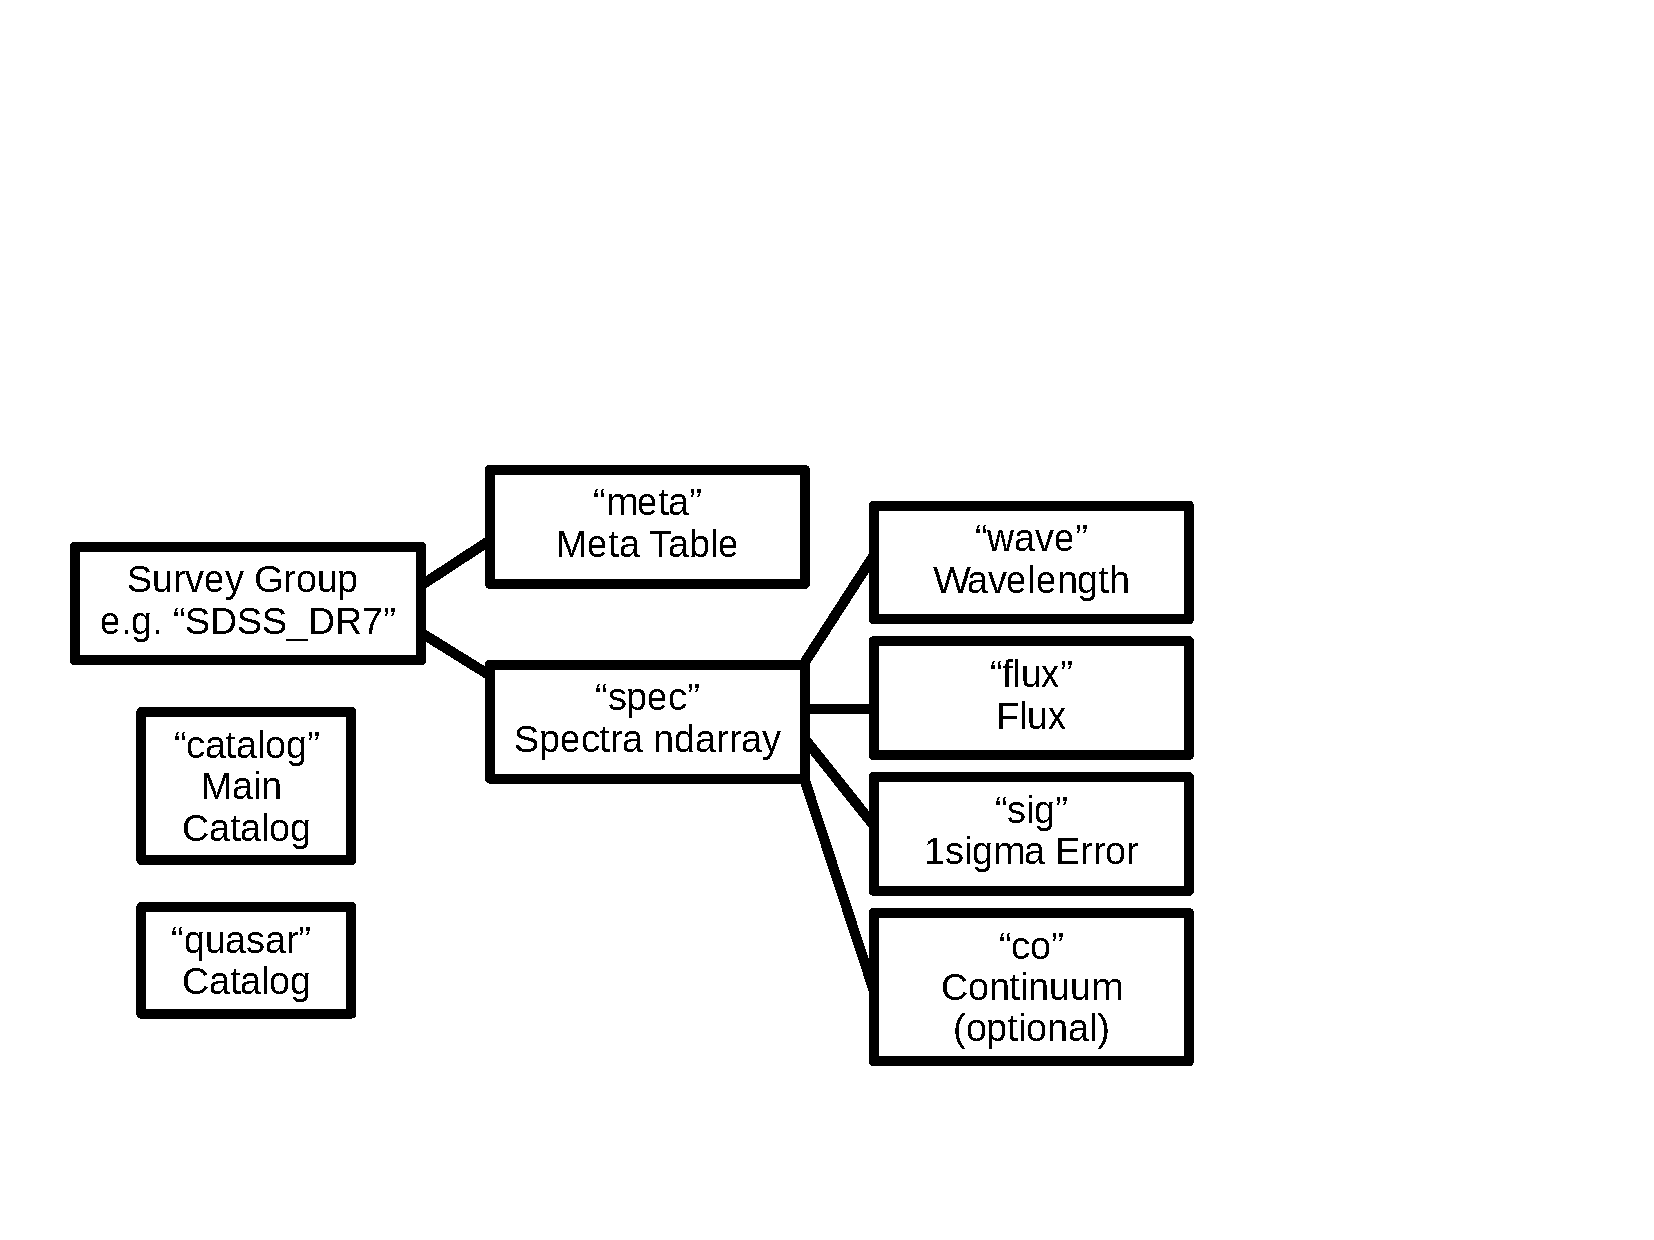
\includegraphics[width=6in]{architecture_v02.pdf}
\caption{igmspec architecture
}
\label{fig:arch}
\end{figure}


\end{document}
